\documentclass[12pt,a4paper]{article}
\usepackage[spanish,es-tabla]{babel}
\usepackage{subcaption} 
\usepackage[utf8]{inputenc} % Escribir con acentos, ~n...
\usepackage{eurosym} % s´ımbolo del euro
\newcommand{\horrule}[1]{\rule{\linewidth}{#1}} % Create horizontal rule command with 1 argument of height
\usepackage{listings}             % Incluye el paquete listing
\usepackage[cache=false]{minted}
\usepackage{graphicx, float} %para incluir imágenes y colocarlas
\usepackage{epstopdf}


\usepackage{hyperref}
\hypersetup{
	colorlinks,
	citecolor=black,
	filecolor=black,
	linkcolor=black,
	urlcolor=black
}
\usepackage{multirow}
\usepackage{array}
\usepackage{diagbox}


\title{
\normalfont \normalsize 
\textsc{{\bf Aprendizaje Automático (2018-2019)} \\ Grado en Ingeniería Informática \\ Universidad de Granada} \\ [25pt] % Your university, school and/or department name(s)
\horrule{0.5pt} \\[0.4cm] % Thin top horizontal rule
\huge 
Reconocimiento de dígitos manuscritos sobre soporte digital \\ % The assignment title
\horrule{2pt} \\[0.5cm] % Thick bottom horizontal rule

\includegraphics{images/logo.png}	
}

\author{Antonio Jesús Heredia Castillo \\ Jose Manuel Perez Lendinez} % Nombre y apellidos

\date{\normalsize\today} % Incluye la fecha actual

%----------------------------------------------------------------------------------------
% DOCUMENTO
%----------------------------------------------------------------------------------------

\begin{document}

\maketitle % Muestra el Título
\newpage %inserta un salto de página
\tableofcontents % para generar el índice de contenidos
\listoffigures
\listoftables
\newpage

\section{Definición del problema a resolver y enfoque elegido}
El problema que hemos elegido es la del reconocimiento de dígitos escritos a mano. Estos dígitos a diferencia de otros dataset, están recogidos sobre soporte digital. \\ Se recogieron muestras de 44 escritores que escribieron 250 dígitos cada uno. Para ello se uso una ``tableta'' de escritura WACOM PL-100V, la cual es sensible a la presión, pero esta característica no fue incorporada en los datos. Se les pidió a los escritores que escribieran 250 dígitos en orden aleatorio dentro de unas cajas sobre la ``tableta'' con una medida de $500\times500$ pixeles. Si los escritores se equivocaban o no estaban contentos con el resultado del dígito podían eliminar el contenido de la caja y realizar de nuevo el dígito. Ademas los 10 primeros digitos son ignorados ya que se usan para que los escritores se acostumbren a la escritura sobre esta tableta, aunque no son informado sobre esto.\\\\
Una forma de visualizar los datos, para hacernos una idea de como están distribuidos es usar la técnica \textbf{t-sne} (T-distributed Stochastic Neighbor Embedding), una tecnica eficaz para reducir la dimensión. Aclaro que esto no lo vamos a usar para reducir la dimensión a la hora de entrenar los modelos, simplemente como forma de poder mostrar un grafico con la distribución de clases. La idea que subyace en esta técnica es que los puntos cercanos se atraen y los lejanos se repelen. Para ello usa un parámetro llamado \textbf{perplexity} que es la cantidad de vecinos que afectan a un determinado punto. Tambien hay una variable \textbf{epsilon} que sera la tasa de aprendizaje, funciona igual que en el descenso del gradiente. Una tasa grande dará pasos muy grandes y no podrá converger y una tasa pequeña tardara mucho mas en llegar. La representación 2D de los datos con t-sne la podemos ver en la Figura \ref{fig:tsne}
\begin{figure}[H]
	\centering
	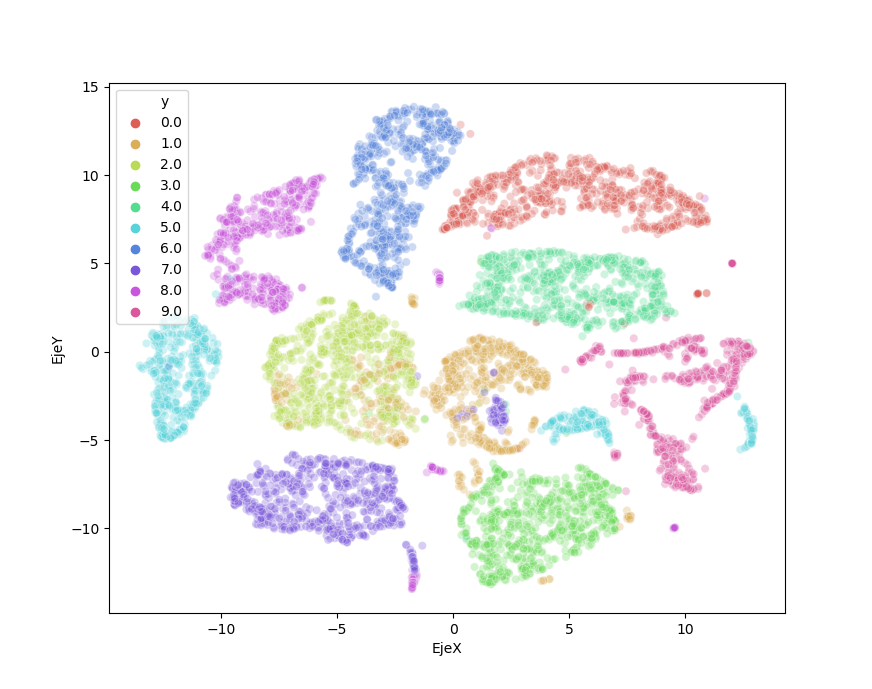
\includegraphics[scale=0.5]{images/tsne.png}
	\caption[Representación con t-sne de los datos]{Representación con t-sne de los datos.}
	\label{fig:tsne}
\end{figure}
Los datos sin procesar que recoge la tableta son las coordenadas $(x,y)$. Estas coordenadas se recogen con una misma separación espacial. Podemos ver un ejemplo de un dígito escrito en la tableta con la información que esta nos pasa y sin procesar en la Figura \ref{fig:digito8Raw} y en la Figura \ref{fig:digito1Raw}.

\begin{figure}[H]
	\centering
	\begin{subfigure}[b]{0.4\textwidth}

		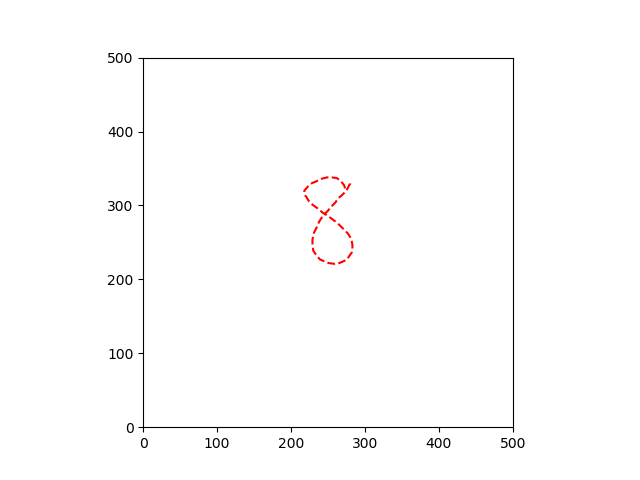
\includegraphics[width=\textwidth]{images/digito8raw.png}
		\caption[Digito ocho recogido por la tableta]{}
		\label{fig:digito8Raw}
	\end{subfigure}
	%
	\begin{subfigure}[b]{0.4\textwidth}

	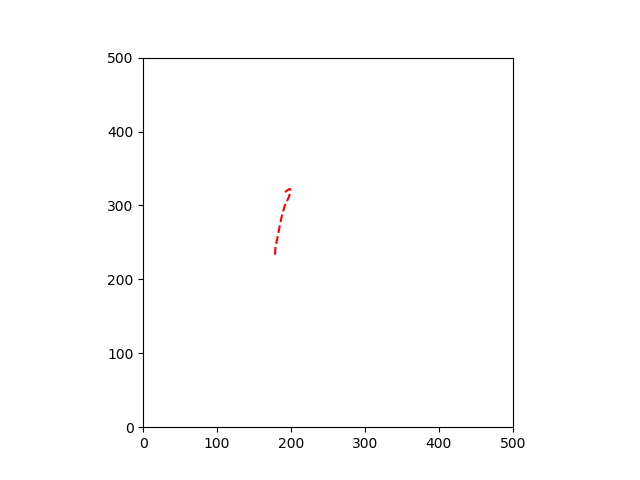
\includegraphics[width=\textwidth]{images/digito1Raw.png}
	\caption[Digito uno recogido por la tableta y sin procesar]{}
	\label{fig:digito1Raw}
	\end{subfigure}
	\caption[Digito ocho y uno recogidos por la tableta]{Datos sin procesar.}
\end{figure}

\section{Codificación de los datos de entrada para hacerlos útiles a los algoritmos.}
Pero como no todos los números tardan lo mismo en escribirse, no todos tendrán la misma cantidad de puntos recogidos. Para ello los proveedores del dataset, realizan una transformación a los datos recibidos por la tableta. Para ello realizan una normalización y remuestree de los datos. Las nuevas coordenadas ahora estarán en un rango entre $(0,100)$ en vez de entre $(0,500)$ como estaban antes. Primero se realiza normalización para asegurarnos que la representación no va a variar con traslaciones o escalados. El remuestreo lo realizan usando una simple interpolación lineal  entre pares de puntos. Ahora se representaran espaciados regularmente en la longitud del arco a diferencia de la secuencia de entrada que esta espaciada regularmente en el tiempo. Los digitos anteriores una vez transformados quedarían como se pueden ver en la Figura \ref{fig:digito8Escalado} y en la Figura \ref{fig:digito1Escalado}

\begin{figure}[H]
	\centering
	\begin{subfigure}[b]{0.4\textwidth}
		
		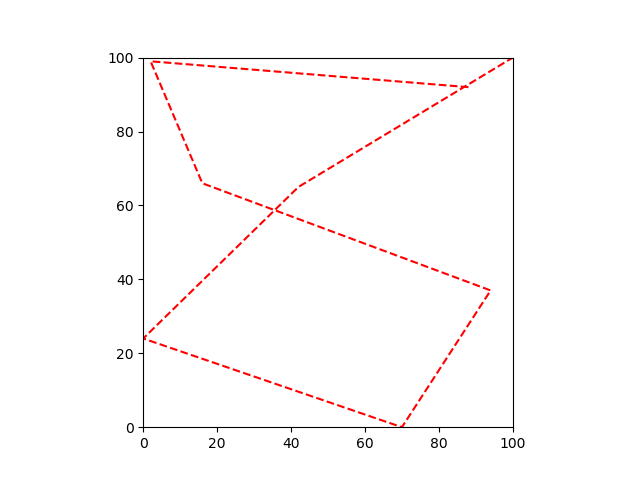
\includegraphics[width=\textwidth]{images/digito8Escalado.png}
		\caption[Digito ocho recogido por la tableta y procesado]{}
		\label{fig:digito8Escalado}
	\end{subfigure}
	%
	\begin{subfigure}[b]{0.4\textwidth}
		
		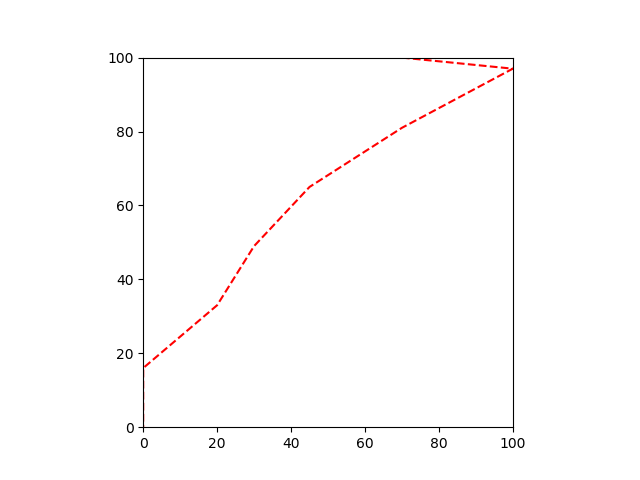
\includegraphics[width=\textwidth]{images/digito1Escalado.png}
		\caption[Digito uno recogido por la tableta y procesado]{}
		\label{fig:digito1Escalado}
	\end{subfigure}
	\caption[Digito ocho una vez realizada la transformación]{Datos una vez procesados.}
\end{figure}

\section{Elección de conjuntos de entrenamiento, test y validación.}

Como en esta practica tenemos que comparar el resultado de distintos modelos. Hemos decidido separar los dato sen tres conjuntos diferentes. El primero sera el de entrenamiento, que como su nombre indica sirve para entrenar el modelo. El segundo sera el de test, este conjunto sirve para ver que tal se ha entrenado nuestro modelo y ver si se ha producido sobreajuste o poder realizar tunning en los parámetros para poder minimizar el error fuera de la muestra. Y por ultimo tenemos el conjunto de validación, en nuestro caso lo usaremos para comparar los distintos modelos. 
\\Haremos una separación en que el  $51.14\%$ de los datos irán al entrenamiento.  El $17.04\%$ irán a validación. Y el resto, que es el $31.82\%$ irán al conjunto de test.\\En esta separación de datos, ademas nos aseguramos que los escritores solo pueden estar en un conjunto. Esto nos puede beneficiar a la hora de que si obtenemos un buen resultado con el conjunto de test podemos asegurar que el modelo a generalizado bien y no a aprendido solo al tipo de escritura de ciertos escritores.


\section{Regresión logística(RL)}	
En este caso nos hemos decantado por RL porque fue el modelo que mejor resultados nos dio en la practica pasada, y al ser un dataset de datos que trata un modelo parecido podremos utilizar los conocimientos previos para mejorarlo. En este caso como el problema es multiclase se ha utilizado one vs rest para clasificar. Vamos a realizar una pequeña explicación de como funciona.

Vamos a poner un pequeño ejemplo con tres clases para ver como funcionaria. Como se ve en la siguiente imagen es imposible dividir las clases con una única linea. 
\begin{figure}[H]
	\centering
	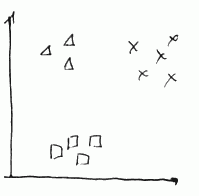
\includegraphics[width=0.7\linewidth]{../imagenesRL/screenshot002}
	\caption{Conjunto de clases}
	\label{fig:screenshot002}
\end{figure}

En las siguientes imágenes se ve como enfrentamos una clase a las otras dos de forma que si se puede conseguir una separación mediante una función lineal.



\begin{figure}[H]
	\centering
	\begin{subfigure}[b]{0.3\textwidth}
		\label{f:gato}
		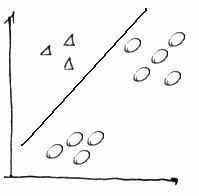
\includegraphics[width=\textwidth]{../imagenesRL/screenshot001}
		\caption[Clasificación de triangulos]{Clasificación de triangulos}	
	\end{subfigure}
	\begin{subfigure}[b]{0.3\textwidth}
		\label{f:tigre}
		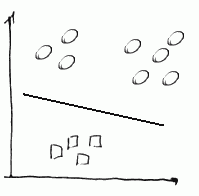
\includegraphics[width=\textwidth]{../imagenesRL/screenshot004}
				\caption[Clasificación de cuadrados]Clasificación de cuadrados{}	
		\end{subfigure}
	\begin{subfigure}[b]{0.3\textwidth}
		\label{f:conejo}
		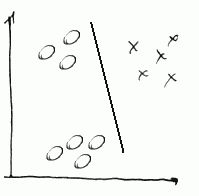
\includegraphics[width=\textwidth]{../imagenesRL/screenshot005}
		\caption[Clasificación de cruces]{Clasificación de cruces}		
\end{subfigure}
	\caption[One vs Rest]{División mediante one vs rest}
\end{figure}

\subsection{Especificación de parámetros RL}
Los parametros a tener en cuenta son:
\begin{enumerate}		
	\item{Umbral de parada:} Indicara cuando tengamos un error menor al indicado pararemos.
	\item{Numero de iteraciones máxima:} En este caso sera en numero máximo de iteraciones podrá realizar si no decide parar antes por el umbral de parada.
\end{enumerate}
Para estos parámetros hemos utilizados los valores por defecto dados por la librería sklean con la que se ha realizado la practica. En este caso el numero de iteraciones esta fijado a 100, aunque suele parar antes sobre unas 30 o 40 iteraciones y el umbral de parada esta inicializado a $10^{-4}$.

En este caso se han realizado pruebas para obtener el mejor parámetro(C) para la regularización. Este parámetro a medida que aumenta realiza una regularización mas suave. También se han realizado pruebas con dos tipos de regularización, que son la L1 y L2. Se han realizado medidas entre 0 y 100 en una serie de dos en dos.

\begin{figure}[H]
	\centering
	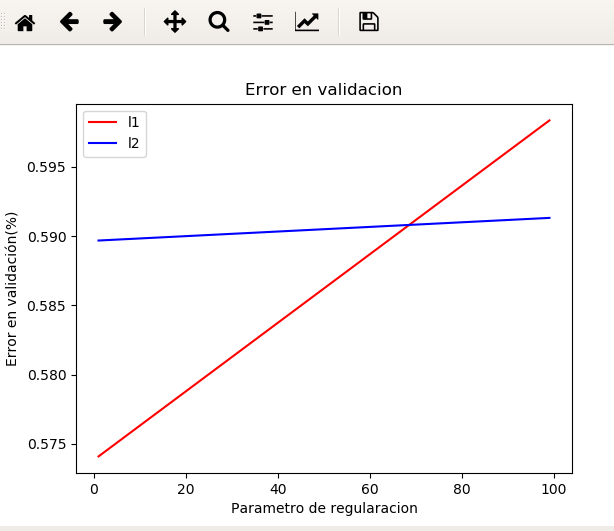
\includegraphics[width=0.7\linewidth]{../imagenesRL/graficaRegularizacion}
	\caption[Regularización en regresión lineal]{Regularización en regresión lineal}
	\label{fig:Grafica de regularizacion}
\end{figure}

En este caso se ve como l1 consigue superar a l2 a la hora de ajustar el error en la partición de validación aunque la mejora solo son en torno a un 0.03\%. En este caso no es muy notorio. El problema viene dado a la hora de tener en cuenta el tiempo de ejecución entre una y otra. 
\begin{figure}[H]
	\centering
	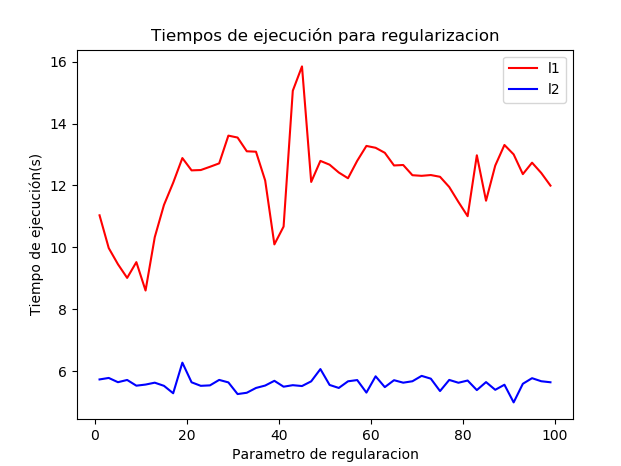
\includegraphics[width=0.7\linewidth]{../imagenesRL/tiemposEjecucion}
	\caption[Tiempo de ejecución regresión lineal]{Tiempo de ejecución regresión lineal}
	\label{fig:tiemposejecucion}
\end{figure}
En este caso l2 es bastante superior a l1. Por estos motivos he decido un parámetro C de 100 y utilizar la regularización de L2.

\subsection{Valoración de resultados}
En este caso para le medición del error se ha utilizado es el mean accuracy.
Se consigue en la partición de test un Eout del 2.3727\% en un tiempo de 4.9801 segundos. Vamos a revisar la matriz de confusión para ver mas información.

\begin{figure}[H]
	\centering
	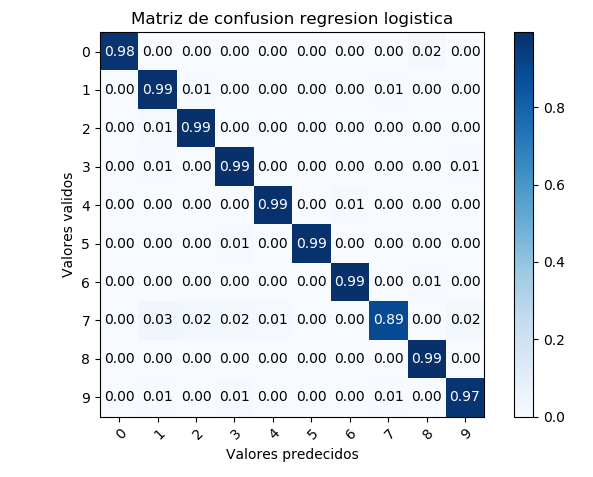
\includegraphics[width=0.7\linewidth]{../imagenesRL/matrizconfusion}
	\caption[Matriz de confusión para regresión lineal]{Matriz de confusión para regresión lineal}
	\label{fig:Matriz confusion RL}
\end{figure}

En este caso se tiene un 10\% errores al adivinar el numero 7, confundiendo este con 1, 2 y 3 . Esto haría que aunque el modelo en geneal tenga un buen acierto se tenga problemas al equivocarnos a menudo en el numero 7.


\section{Redes neuronales}
Hemos relizado un modelo con redes neuronales. Para ello hemos usado al librería ``Keras'' que nos dejaba mucho margen a la hora de configurar la rede neuronal. No solo te permite decir la cantidad de capas ocultas que tiene si no que ademas te permite especificar cuantas neuronas tendrá cada capa, para así ajustar mejor tu modelo. Otras librerías como Scikit-Learn no te permiten tener un numero distinto de neuronas por capa, si no que todas las neuronas tienen que tener la misma cantidad.

\subsection{Elección de la mejor configuración para la red}
Para este modelo tenemos como capa de entrada 16 neuronas, que corresponde con cada una de las características de entrada de nuestro modelo. Como capa de salida tendremos diez neuronas. Esto se hace así, ya que según la neurona que se active clasificara un numero u otro. Cuando clasifica por ejemplo el dígito 0, activara la neurona numero ``cero'' y las demás las dejara con un valor muy próximo a cero. Nuestra red tendrá una parecía parecida a la que podemos ver en la Figura \ref{fig:redneuronal}
\begin{figure}[H]
	\centering
	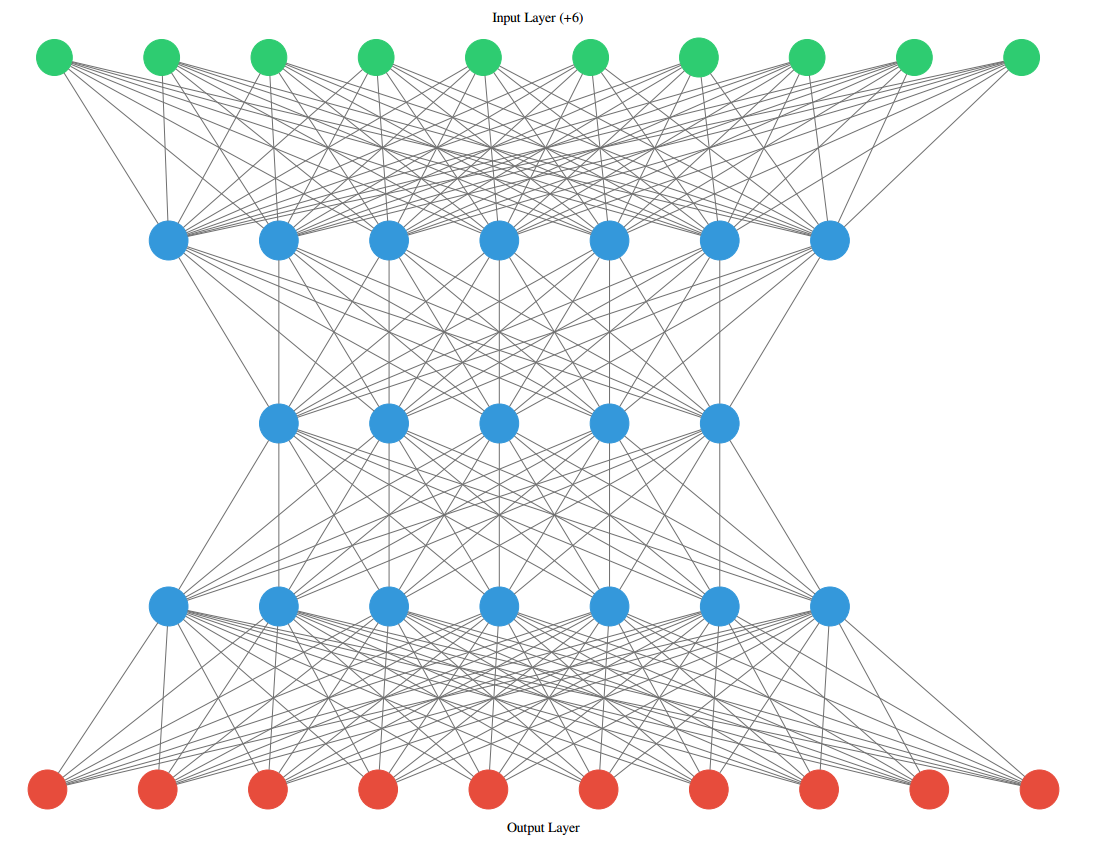
\includegraphics[width=0.7\linewidth]{images/redNeuronal}
	\caption[Modelo de red neuronal]{}
	\label{fig:redneuronal}
\end{figure}

Para ver como afectaba la cantidad de neuronas por capa a nuestro modelo he realizado un pequeño experimento en el que iba aumentando la cantidad de neuronas y comprando las dos funciones de actividad mas comunes ``relu'' y ``sigmoide''. Como función de activación en la ultima capa he usado ``SoftMax'' ya que es una de las que mejores funcionan con el modelo de tener que activar neuronas en la ultima capa para saber a que clase pertenecen los datos. En la Figura \ref{fig:comparacionReuluSigmo} podemos ver la comparación entre las dos funciones de activación que hemos comentado. En verde podemos ver ``Sigmoid'' y en rojo ``relu''. 
\begin{figure}[H]
	\centering
	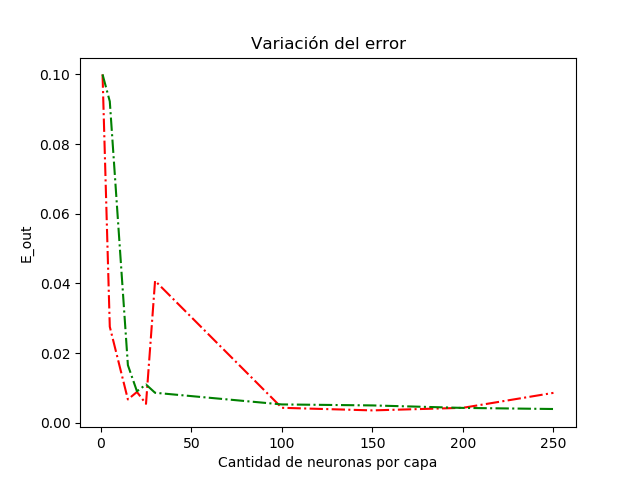
\includegraphics[width=0.7\linewidth]{images/comparacionreluSigmo.png}
	\caption[Comparación entre Sigmoid y relu]{Comparación entre Sigmoid y relu}
	\label{fig:comparacionReuluSigmo}
\end{figure}
Como podemos ver con un numero grande de neuronas las dos funcionan de forma parecida. Pero en cambio con un numero de neuronas entre 20 y 100 relu parece funcionar de forma extraña. Por ello he elegido para nuestro modelo usar sigmoid  y un numero de neuronas por capa de 20. Aunque podría haber obtenido resultados un poco mejores con mas numero de neuronas, la diferencia era casi mínima. Por ello elegí una pequeña cantidad de neuronas, para tener el modelo mas simple posible e intentado que no sobreajustara.
\subsection{Valoración de los resultados}
Para ver como ha funcionado nuestro modelo hemos usado la media de aciertos. Hemos obtenido un $E_{out}=0.029$. Viendo estos resultados podemos deducir que el modelo ha generalizado de forma correcta y es capaz de predecir la mayoría de los datos pasados en el test. Esto se puede observar de forma mas directa en la matriz de confusión. Viendo que tiene muy pocas malas prediciones.
\begin{figure}[H]
	\centering
	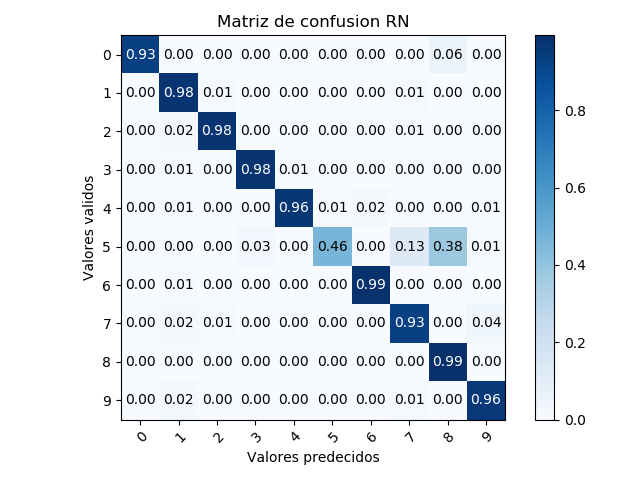
\includegraphics[width=0.7\linewidth]{images/confusionMatrixRN.png}
	\caption[Matriz de confusión para redes neuronales]{Matriz de confusión para redes neuronales}
	\label{fig:MatrizConfusio0nRN}
\end{figure}
\section{Random forest(RF)}	
Se usa esta técnica puesto que es un muy buen clasificador. En este caso al meter información extra a el dataset tendremos una cantidad grande de variables y esta técnica trabaja muy bien cuando se tienen gran numero de variables.
\subsection{Especificación de parámetros RF} 
En este caso nos hemos centrado en la elección de una buena cantidad de arboles y la cantidad de variables que utilizara cada árbol para predecir. Para seleccionar estos parámetros se han realizado varias pruebas con la partición de validación. Se ha medido el error con la partición de validación con tres cantidades distintas de variables. El numero de variables elegidas para cada una son las siguientes:
\begin{enumerate}
	\item Raíz: En este caso se tendrá una cantidad de características para cada árbol igual a la raíz cuadrada del numero de características. 
	\item Mitad: La cantidad de variables sera en esta opción la mitad de las características.
	\item Cantidad de características: Para esta opción cada árbol utilizara todas las características.
\end{enumerate}

El numero de arboles lo iremos aumentando de 10 en 10 hasta llegar a 250. 

Pasamos a mostrar el grafico para analizar el mejor numero de características para utilizar.
\begin{figure}[H]
	\centering
	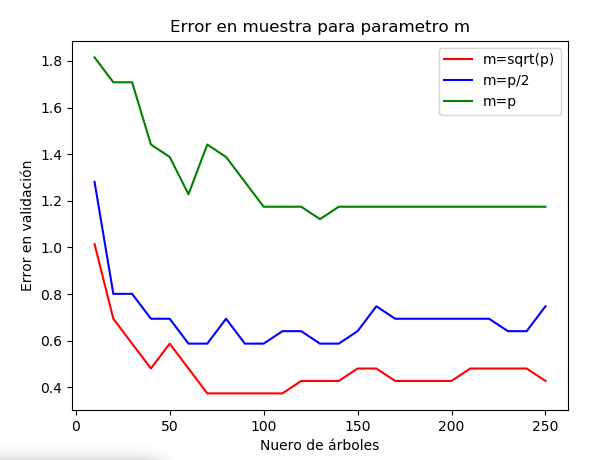
\includegraphics[width=0.7\linewidth]{../imagenesRF/errorvalidacion}
	\caption[Cantidad de variables Random Foreset]{}
	\label{fig:Cantidad de variables RF}
\end{figure}
En el grafico se ve claramente que la mejor opción es la raíz. También podemos sacar de este grafico cual es la mejor opción para el numero de arboles necesarios. En este caso a partir de 70 se tiende a igualar y no mejora. Para decidirnos por el numero de arboles tendremos en cuenta también el siguiente grafico, donde se muestra el tiempo de ejecución para cada cantidad de arboles.

\begin{figure}[H]
	\centering
	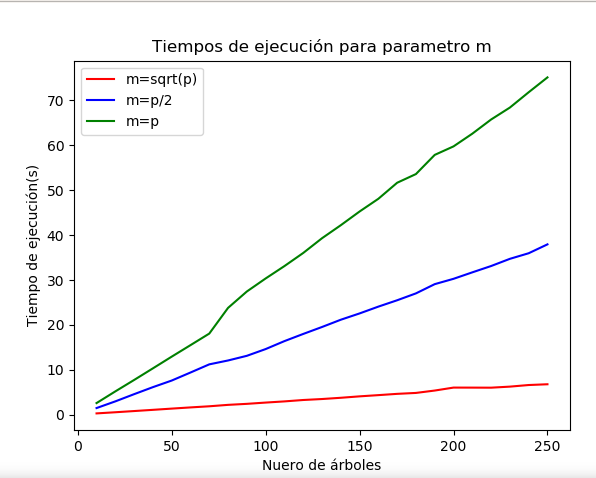
\includegraphics[width=0.7\linewidth]{../imagenesRF/tiempoEjecucion}
	\caption[Tiempos de ejecución]{Tiempos de ejecución}
	\label{fig:tiempoejecucion}
\end{figure}

En este caso se ve que con mas cantidad de arboles tendremos una mayor tiempo de ejecución. Por tanto he decido definir la cantidad de arboles a 100 y quedarme con la opción de la raíz para el numero de características por árbol.


\subsection{Valoración de resultados}
La métrica utilizada en este caso es mean accuracy y el error obtenido en la partición de test es el 3.5162 \%. En este caso no es un mal porcentaje de error pero vamos a analizar la matriz de confusión para tener una mejor idea.

\begin{figure}[H]
	\centering
	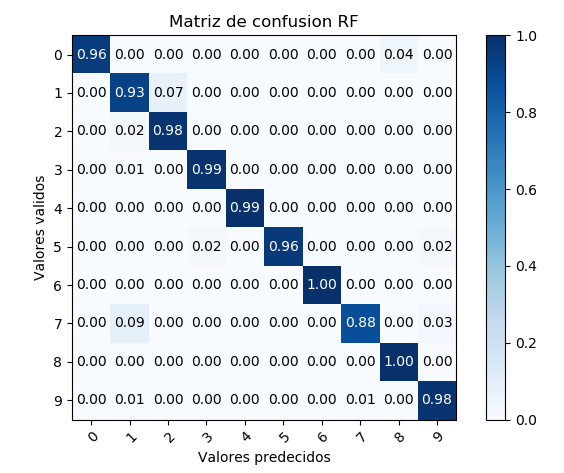
\includegraphics[width=0.7\linewidth]{../imagenesRF/matrizConfusion}
	\caption[Matriz de confusión Random Forest]{Matriz de confusión Random Fores}
	\label{fig:MatrizDeConfusionRF}
\end{figure}

En este caso se ve que tenemos falla mucho al prediciendo 7 como 1 y también confunde los 1 con 2. Esto nos podría llegar a fallar mas de lo común en el reconocimiento de estos dígitos.

En este caso he querido utilizar una partición de validación en vez de utilizar el método de oob para la validación, por realizarlo de la misma manera que los modelos anteriores.

\section{Support Vector Machine}
Para el modelo de SVM hemos utilizado la libreria de Scikit-Learn. Como en los enunciados nos daban a elegir entre usar un kernel \textbf{polinomico} o \textbf{RBF}, hice pruebas con los dos y llegue a la conclusión de que \textbf{RBF} me producia mucho sobre ajuste, ya que me daba un error de cero en el entrenamiento pero en la muestra me daba un error de mas de $0.8$. Por lo tanto el modelo para estos datos lo he relizado con un kernel \textbf{polinomico}.
\subsection{Especificación de parámetros SVM}
Cuando utilizamos un kernel polinomico, hay dos variables mas que afectan a nuestro modelo. El primero es el grado del polinomio. Para ver que grado nos daba mejor resultado en nuestro problema hemos realizado un una serie de pruebas para ver cual ajusta mejor. Hemos probado grados desde el 0 hasta el 10 y podemos ver los resultados en la Figura \ref{fig:errorsvm}
 \begin{figure}[H]
 	\centering
 	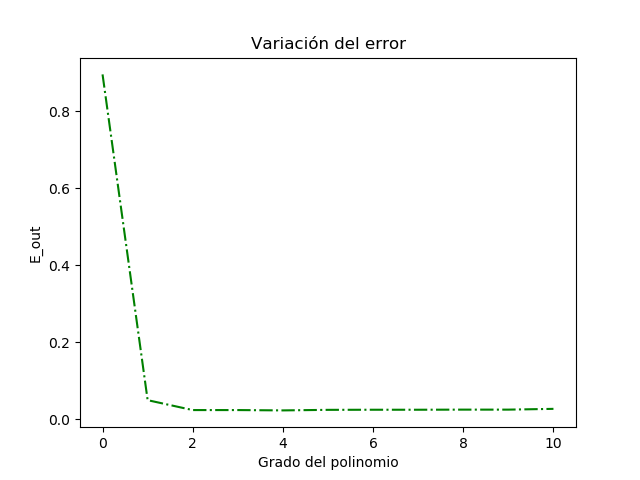
\includegraphics[width=0.7\linewidth]{images/errorsvm.png}
 	\caption[Variación del error en función del grado del polinomio]{Variación del error en función del grado del polinomio}
 	\label{fig:errorsvm}
 \end{figure}
Como podemos ver, el modelo a partir de grado 2 obtiene siempre un error muy parecido, por lo tanto hemos seleccionado grado 2, ya que a igualdad de resultados siempre es mejor coger el modelo mas simple. \\\\
El otro parámetro que influye es el coeficiente independiente, para este coeficiente también he realizado pruebas, a ver con cual iba mejor nuestro modelo. Realice una serie de ejecuciones con coeficiente desde 0 hasta 100. El resultado de estas pruebas lo podemos ver el la Figura \ref{fig:errorCoeficientesvm}
 \begin{figure}[H]
	\centering
	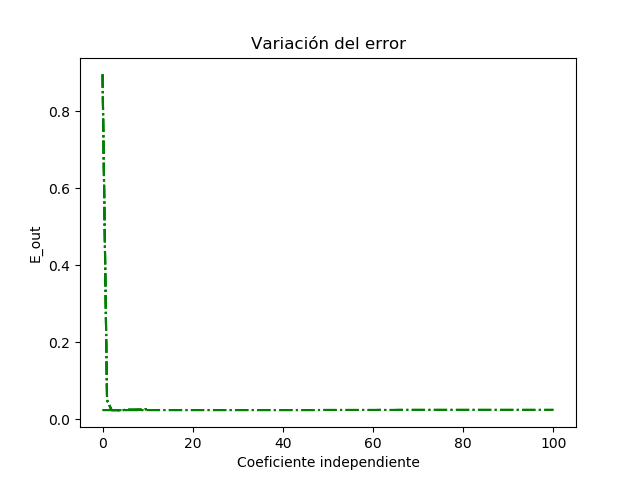
\includegraphics[width=0.7\linewidth]{images/errorCoefIndependietesvm.png}
	\caption[Variación del error en función del coeficiente independiente]{Variación del error en función del coeficiente independiente}
	\label{fig:errorCoeficientesvm}
\end{figure}
Al igual que pasaba con el grado del polinomio, llega un momento en el que se estabiliza el error, esto ocurre a partir del coeficiente 5, por lo tanto ese sera el coeficiente independiente que elegiremos para nuestro modelo.
\subsection{Valoración de resultados}
Usando un grado del kernel polinomico de cuatro y un coeficiente independiente de 5, hemos conseguido un  $97.57\%$ sobre los datos de test. Esto se traducen en un $E_{out}=0.0343$, por lo tanto estamos ante un modelo que ajusta bastante bien a nuestros datos y que tiene una buen generalización. Estos datos se pueden observar mejor en la matriz de confusión (Figura \ref{fig:matrizConfusionSVM})y ver en que numeros ha tenido mas fallos y en cuales menos. 
 \begin{figure}[H]
	\centering
	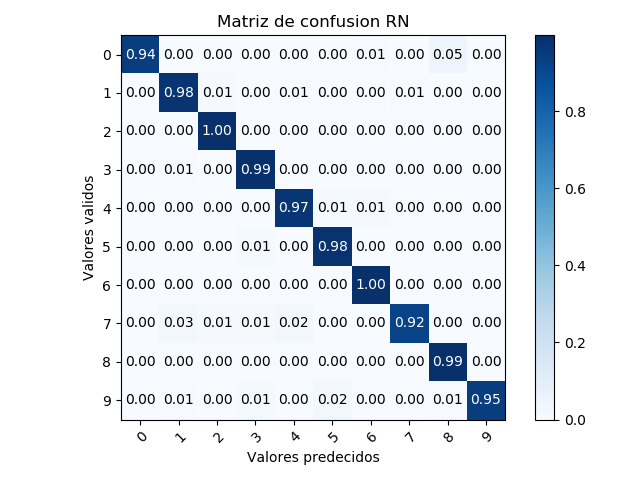
\includegraphics[width=0.7\linewidth]{images/confusionmatrixsvm.png}
	\caption[Matriz de confusion para SVM]{Matriz de confusion para SVM}
	\label{fig:matrizConfusionSVM}
\end{figure}
\section{Comparación de modelos}
Para comparar los distintos modelos hemos visto cual es el error con los distinto modelos en la partición de validación. Hemos recogido los distintos errores en una tabla para poder ver cual es menor y ese sera con el que nos quedemos.\\\\
\begin{tabular}{|c|c|c|c|c|}
	\hline 
	& Regresión Lineal & SVM & Random Forest & Redes Neuronales \\ 
	\hline 
	Error & 0.00587 & 0.0069 & 0.3737 & 0.0040 \\ 
	\hline 
\end{tabular}\\\\
Viendo los datos, el modelo que nos da un mejor resultado son las Redes Neuronales, aunque podriamos usar igualmente regresión lineal o support vector machine, ya que nos da resultados muy parecidos. El modelo que parece funcionar un poco peor con nuestro dataset seria Random Forest. 
\end{document}